
\textbf{\underline{В первой главе}} представлены обзоры и анализы областей, которые необходимы для решения поставленных научных задач.

Была проведена классификация машин, использующих ноги в качестве движителя. Это необходимо для понимания места объекта исследования среди других роботов, а также понимания типичных ошибок, которые возможно совершить при разработке. По результатам классификации объектом исследования является многоногая шагающая машина с движителями циклического действия.

Рассмотренные роботы этого класса были изучены и их ключевые особенности внесены в таблицу, что позволило понять структурные и габаритные особенности данного класса роботов. К примеру, длинна таких роботов обычно не превышает 1 метр, а количество ног может варьироваться от 4-ех до 32-ух.

Так как основным местом применения разработанных методов предполагается исследование пещер роботами, то были рассмотрены типы роботов и робототехнических систем, которые могут использоваться для изучения поверхности пещер. Изучение данных роботов позволило понять какой функционал и какие габаритные ограничения закладывались их разработчиками.

Таким образом были найдены причины, к примеру типы опорных поверхностей, которые влияют на подбор сенсоров и алгоритмов, а также сделаны выводы о том как это влияет на робототехническую систему. 

На основе опыта, собранного исследователями со всего мира, были выбраны технически решения, связанные с навигацией, выбором сенсоров и архитектурными решениями, представленные далее

Для решения задачи определения геометрических и физико-механических свойств пройденной поверхности необходимо понимать в каких условиях будет использоваться робот. В пещерах встречаются следующие типы поверхностей: твердые породы, прочные (мрамор), мягкие (мел, известняк); сыпучие грунты (песок); водные преграды (лужи, бассейны); скользкие и упругие поверхности (мох, плесень); пластинчатые (земля). Было решено сделать упор на твердые, упругие и пластинчатые поверхности.

Так же были рассмотрены размеры пещер, чтобы понимать необходимый запас хода, размеры робототехнического комплекса, также чтобы понимать минимальную достаточную точность построения карты. Длины многих пещер измеряются километрами, а их габариты очень сильно варьируются от нескольких сантиметров, до многих километров в ширину.

В основе автономной навигации роботов лежат Simultaneous Localization and Mapping (SLAM) методы. Так как задача определения геометрических свойство объекта является одной из частью данного метода (Mapping), то были рассмотрены алгоритмы, основанные на использовании камеры, стереопары, с использованием лидара, GPS, IMU а также их различные комбинации. Было решено решать задачу локализации с помощью маяков или ToF камеры, а для построения карты разработать свой метод.

Так как предполагался метод построения карты с помощью ощупывания поверхности, то был произведен поиск подобных алгоритмов. Были найдены способы получения облака точек объекта с помощью касания манипулятором данного объекта. Примерное местоположение объекта определялось камерой.

Проведен обзор алгоритмов триангуляции, так как данный метод лёг в основу определения геометрических свойств объекта. Было решено модифицировать 2D триангуляцию Делоне для вогнутых оболочек.

Рассматривались различные алгоритмы и средства определения физическо-механических свойств поверхности. Этр возможно реализовать с помощью следующих сенсоров сенсоров: камеры, с помощью инерциального измерительного устройства (IMU),  снятия тока с моторов, момента с вала мотора, с помощью датчиков силы, установленных на конечность робота. Было решено выбрать главным сенсором --- датчик силы, установленный на ногу робота, но также собирать дополнительные данные с инерциального измерительного устройства и драйвера мотора: скорость, потребляемый ток.

Для решения задачи структурного синтеза на основе критериев проходимости, детализации и пройденного пути (оптимизация количества ног у робота), необходимо генерировать семейства поверхностей с одинаковой сложностью. Поиск различных вариантов привел к выбору подхода <<Получение искусственных поверхностей на основе параметров генерации>>, который был модифицирован автором.

Для определения геометрических свойств поверхности были  выделены следующие решения:
\begin{itemize}
    \item Построение карты с помощью лидаров и камер;
    \item Получение облака точек с помощью тактильного очувствления манипулятором.
\end{itemize}
Метод построения карты с помощью тактильного очувствления шагающим роботом отличается от представленных выше решений.

Для определения физико-механических свойств был переосмыслен алгоритм классификации типа поверхности пройденной конечностью робота, на которой установлены датчики силы и IMU. Задача классификация решается с помощью алгоритмов машинного обучения.  

На основе литературного обзора было решено, что предложенные решения для определения геометрических и физико-механических свойств не встречается в научных публикациях российских и зарубежных авторов.

Итогом первой главы является обзор разработанной системы \pic{fig:diag_system.png}.
\begin{figure}[ht!]
    \centering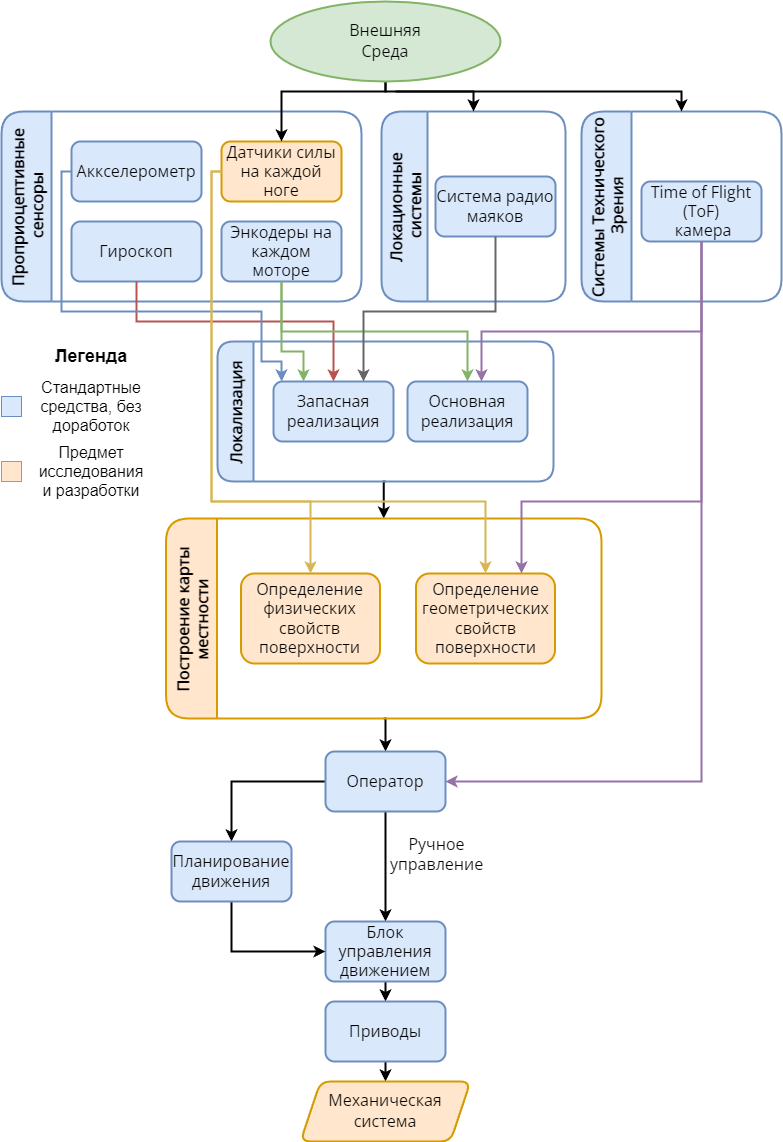
\includegraphics[height=15cm,width=1\textwidth,keepaspectratio]{main_diag.drawio.png}
    \caption{Структурная схема разработанной системы}
    \label{fig:diag_system.png}
\end{figure}

Оранжевым цветом выделены те компоненты системы, которые представляют собой предмет исследования в рамках диссертационной работы. Их разработка и научная новизна описаны в последующих главах диссертации. Голубым цветом выделены блоки, соответствующие которым элементы в разработанную систему были интегрированы как стандартные средства,   без каких-либо существенных доработок.

Верхний блок --- внешняя среда, то есть вся информация о внешнем мире, с которой работает робот.

Следующая группа представлена <<Проприоцептивные сенсоры>>, то есть внутренними датчиками. Есть группа блоков, посвященная техническому зрению. Последней группой элементов является <<Локационные системы>>, представленные системой радио маяков. 

Ниже находится группа блоков <<Локализация>>. В ней расположены два блока <<Основная реализация>> и <<Запасная реализация>>. Первая является более точной. Она может быть реализована на основе системы радио маяков или с помощью системы технического зрения. Запасная реализация является резервной, когда отказала основная реализация, или когда та выдает некорректные результаты. Она основана на IMU, датчиках силы и системе маяков.

Блок <<Построение карты местности>> позволяет параллельно с исследованием геометрических свойств поверхности, посредством ее ощупывания, определять физико-механические свойства поверхности по которой ходит робот. Построение карты местности объединяет данные с других двух блоков и выводит результат в машино и человеко читабельные виды.

Оператор может управлять роботом, как в ручном режиме, так и задав область, куда роботу нужно прийти. Эта высокоуровневая команда передается в блок управления движением, которая в последствии преобразуется в низкоуровневые команды для приводов робота. С помощью данных команд, механическая система, представленная разработанным роботом приводится в движение и выполняется поставленная оператором задача.
